\chapter{Beobachtung} \label{Beobachtung}
Um ein realistisches Modell erstellen zu können, führte ich empirische Beobachtungen an drei großen Haltestellen der Münchener U-Bahn durch. Für die spätere Auswertung habe ich hierbei Aufnahmen des Fahrgastwechsels angefertigt. Die Anfertigung der Aufnahmen beschreibe ich im Folgenden. 
\section{Aufnahmen der Beobachtung} \label{Aufnahmedetails}
Zum Aufnehmen des Wechselprozesses nahm ich einen Platz auf den an U-Bahn-Stationen vorhandenen Wartebänken ein. Von diesem Platz aus konnte ich bei Einfahren des Zuges immer eine Tür frontal aufnehmen. Eine beispielhafte Skizze, für die Position, aus der ich beobachtete, kann in \figurename \ref{fig:skizzeBeobachtung} betrachtet werden. \\
\begin{figure}[H]
	\centering
		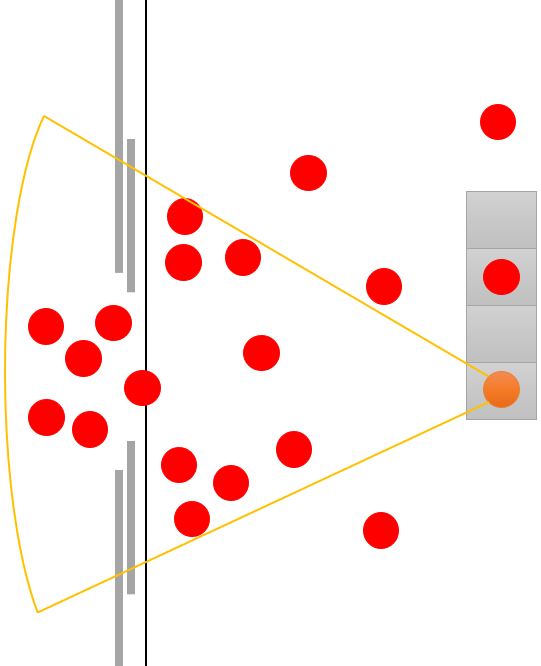
\includegraphics[angle=270, width=0.6\textwidth]{pictures/observation/recording/example_tapping.png}
	\caption{Skizze der Aufnahme an Bahnsteigen aus der Vogelperspektive. Die grauen Rechtecke stellen die Bänke des Bahnhofes dar. Hellgraue Linien zeigen die "`Wände"' des Zuges. Die schwarze Linie zeigt die Bahnsteigkante. Die roten Kreise repräsentieren Fahrgäste, während der orange Punkt die filmende Person darstellt. In Gelb ist der Bereich eingezeichnet, der von der Kamera eingefangen wurde.}
	\label{fig:skizzeBeobachtung}
\end{figure}
Zum Filmen der Türen verwendete ich die Kamera "'Canon EOS 650D"'. Für jeden einfahrenden Zug erstellte ich ein Video. Die Aufnahmen der U-Bahnen fanden zwischen dem 26. März und 25. Mai 2019 statt. Die Aufnahmen fertigte ich dabei zwischen 8:00 und 18:00 Uhr an. Im angegebenen Zeitraum wurden 67 Videos aufgenommen von denen 56 Videos für die Weiterverarbeitung geeignet waren. Auf den anderen Videos stehen Personen derart im Weg, dass eine Auswertung des Fahrgastwechsels nur sehr ungenau oder gar nicht möglich gewesen ist. Somit beobachtete ich 56 Türen, an denen ein Fahrgastwechsel stattfand. Dabei nahm ich 1173 Personen auf Video auf. Die Beobachtung fanden an 3 großen Haltestellen der MVG statt: am Marienplatz München, am Odeonsplatz und am Hauptbahnhof. Während der Beobachtung nahm ich mit einer Kamera auf, wie der Fahrgastwechsel abläuft. Die gefilmten Fahrgäste wurden nicht darüber informiert, dass ich sie beobachtete und aufnahm, um ihr Verhalten nicht zu beeinflussen. Das ist zulässig, weil die Aufnahmen nicht veröffentlicht werden, sondern nur der Datenerhebung dienen. Videos oder Bilder, die der Veranschaulichung dienen, anonymisiere ich vor der Veröffentlichung komplett: auf dem Bildmaterial aufgenommene Personen werden unkenntlich gemacht. In dieser Arbeit verwendete ich zwei Methoden zur Verfälschung der Identitäten. Zum einem bearbeitete ich Bilder mit dem Bildbearbeitungsprogramm \textsf{GIMP}. Bei der Bearbeitung verpixele ich die Gesichter der Personen so, dass diese nicht mehr erkennbar sind. Zudem verwendete ich zur Bearbeitung von Bildern und Videos den Code eines Kommilitonen, Andre Heinrich. Dieser erstellte in einem vergangenen Semester einen Filter in \textsf{Jupyter Notebook} der ein Bild Comic-artig zu Strichzeichnungen vereinfacht.
Die \figurename \ref{fig:PersonenUberZeit} zeigt genauer, zu welchen Zeiten Videos aufgenommen wurden, und wie viele Personen zu diesen Zeiten durchschnittlich am Fahrgastwechsel beteiligt waren.
\begin{figure}[H]
	\centering
		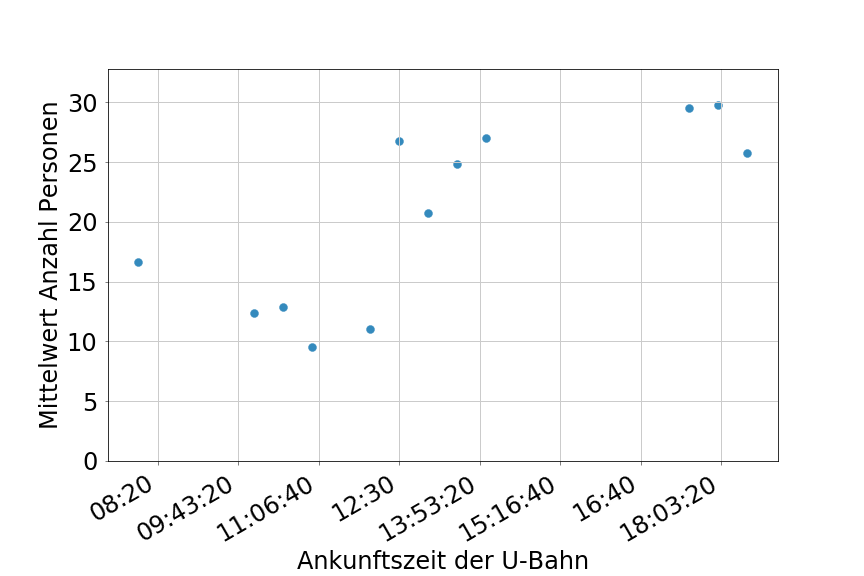
\includegraphics[width=1.0\textwidth]{pictures/observation/recording/peopleOverTime.png}
	\caption{Mittelwert der Anzahl der Beobachteten zu aufgenommenen Zeiten.}
	\label{fig:PersonenUberZeit}
\end{figure}
In diesem Plot kann erkannt werden, dass die höchsten Werte für Anzahl an Personen zwischen 17:00 und 18:00 Uhr erreicht wurden. Dieses Ergebnis stimmt mit den Angaben der Deutschen Bahn überein, welche angibt, dass ihre Hauptverkehrszeiten zwischen 6:30 und 9:30 Uhr sowie 15:30 und 18:30 liegen (\cite{DeutscheBahnAG.2018}). Die hohen Werte zwischen 12:30 und 15:00 wurden am Wochenende aufgenommen. Die Angaben der Deutschen Bahn beziehen sich auf Hauptverkehrszeiten unter der Woche.
\section{Standardfall}
Im Standardfall der Beobachtungen ist ein einigermaßen ausgeglichenes Verhältnis an ein- und aussteigenden Personen gegeben. Wollen Personen in den einfahrenden Zug einsteigen, begeben sie sich in an die Türen der U-Bahn. Wollen auf dem Bahnsteig wartenden Fahrgäste jedoch nicht in diesen Zug einsteigen, so verbleiben diese auf ihrer Position in gewissem Abstand von den Gleisen. Begeben sich die Einsteigenden an den Zug, positionieren diese sich im Normalfall rechts und links der Tür, um den Aussteigenden Platz zu gewähren. Dieser Fall kann in \figurename \ref{fig:normalerFahrgastwechsel} beobachtet werden.
\begin{figure}[H] 
	\centering
		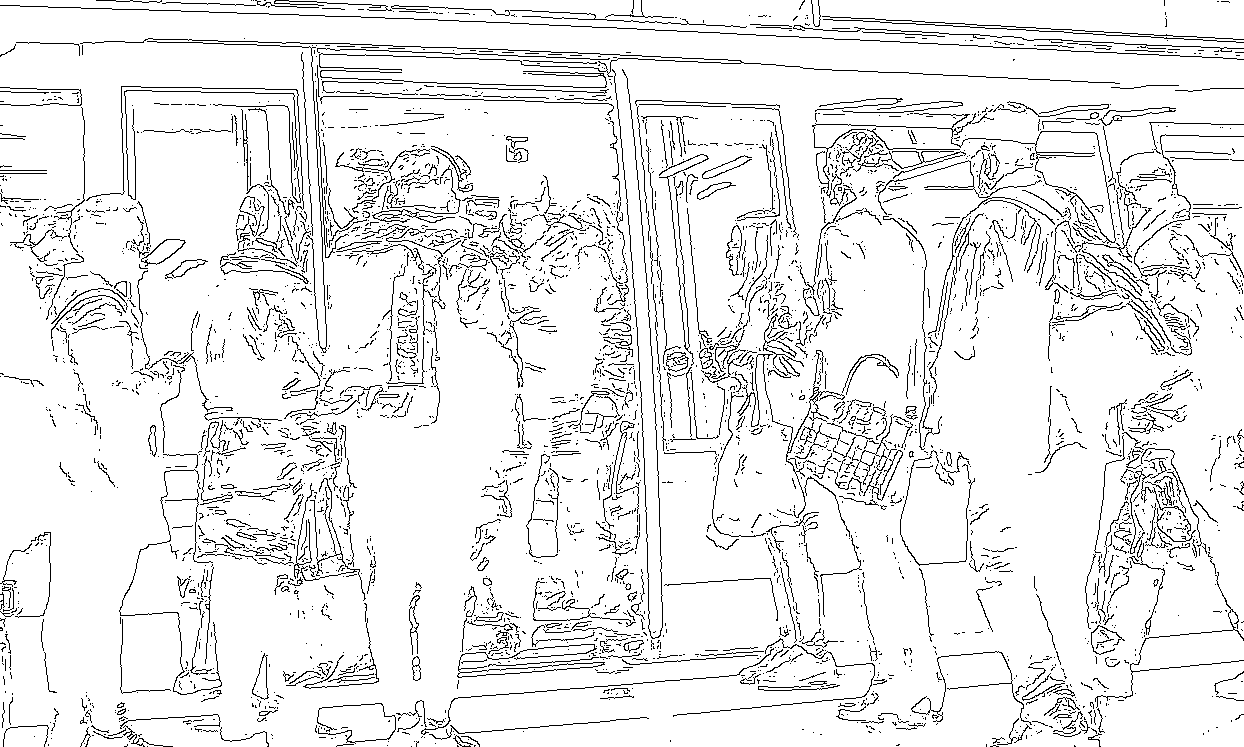
\includegraphics[width=0.8\textwidth]{pictures/observation/standard/exchange.png} 
	\caption{Fahrgastwechsel mit Einsteigern und Aussteigern im Standardfall.}
	\label{fig:normalerFahrgastwechsel}
\end{figure} 
Aussteigende beginnen sich aus dem Zug zu bewegen, wenn die Türen geöffnet werden und steigen normalerweise in Zweierreihen aus dem Zug aus. Im häufigsten Fall beginnen die Einsteiger dann mit dem Einsteigeprozess, wenn alle Aussteigenden aus der Tür ausgestiegen sind.
\section{Sonderfall: Beobachtungen vor einem Fußballspiel} \label{Fussballspiel}
Im Beobachtungszeitraum fand in München ein großes Fußballspiel statt. Einer der Münchner Fußballvereine, der FC Bayern München, spielte am 6. April 2019 gegen den Dortmunder Verein BVB (Ballspiel-Verein-Borussia). Da es mich interessierte, ob sich das Verhalten der Ein- und Aussteiger bei einer solchen Veranstaltung verändert, habe ich an diesem Tag den Fahrgastwechsel beobachtet. Die Beobachtungen fanden an diesem Tag vor Beginn des Fußballspiels statt. Die observierten Personen befanden sich somit auf dem Weg zum Stadion. Einflüsse auf das Verhalten durch das Ergebnis des Spieles konnten somit nicht in die Daten eingehen. Die Unterschiede zu Beobachtungen an Tagen ohne Veranstaltungen werden im Folgenden kurz erläutert und mögliche Erklärungen für diese Unterschiede beschrieben. 
\subsection{Unterschiede}
Zunächst ist zu erwähnen, dass sich das Verhältnis von Einsteigern zu Aussteigern deutlich veränderte. An der beobachteten Station, dem Marienplatz München, stiegen in diesem Zeitraum, trotz vieler Personen im Zug, nur sehr wenige Personen aus.\\ 
Abgesehen vom Unterschied im Verhältnis der Prozesstypen konnte auch eine Veränderung im Verhalten beobachtet werden. Vor dem Fußballspiel positionierte sich ein Großteil der Personen nah am Bahnsteig. Somit standen diese Wartenden auch direkt am Zug, und damit auch an den Türen, wenn sie nicht in den Zug einsteigen wollten.\\
Ein weiterer Unterschied ließ sich darin erkennen, wie Fahrgäste sich an die Türen stellten. In dem beobachteten Zeitraum vor dem Fußballspiel konnte diese Verhaltensweise des rechts und links stehen vor der Tür nicht erkannt werden. Bei dieser Beobachtung standen alle wartenden Personen, direkt am Eingang des Wagons, wie in \figurename \ref{fig:fussballFahrgastwechsel} zu sehen ist. Aussteiger mussten sich einen Weg durch die Masse suchen und konnten nicht auf geradem Weg den Zug verlassen. Auch die zuvor beschriebenen Personen, welche nicht in den Zug gelangen wollten, versperrten somit einen Großteil des Weges für Aussteigende. \\
\begin{figure}[H]
	\centering
		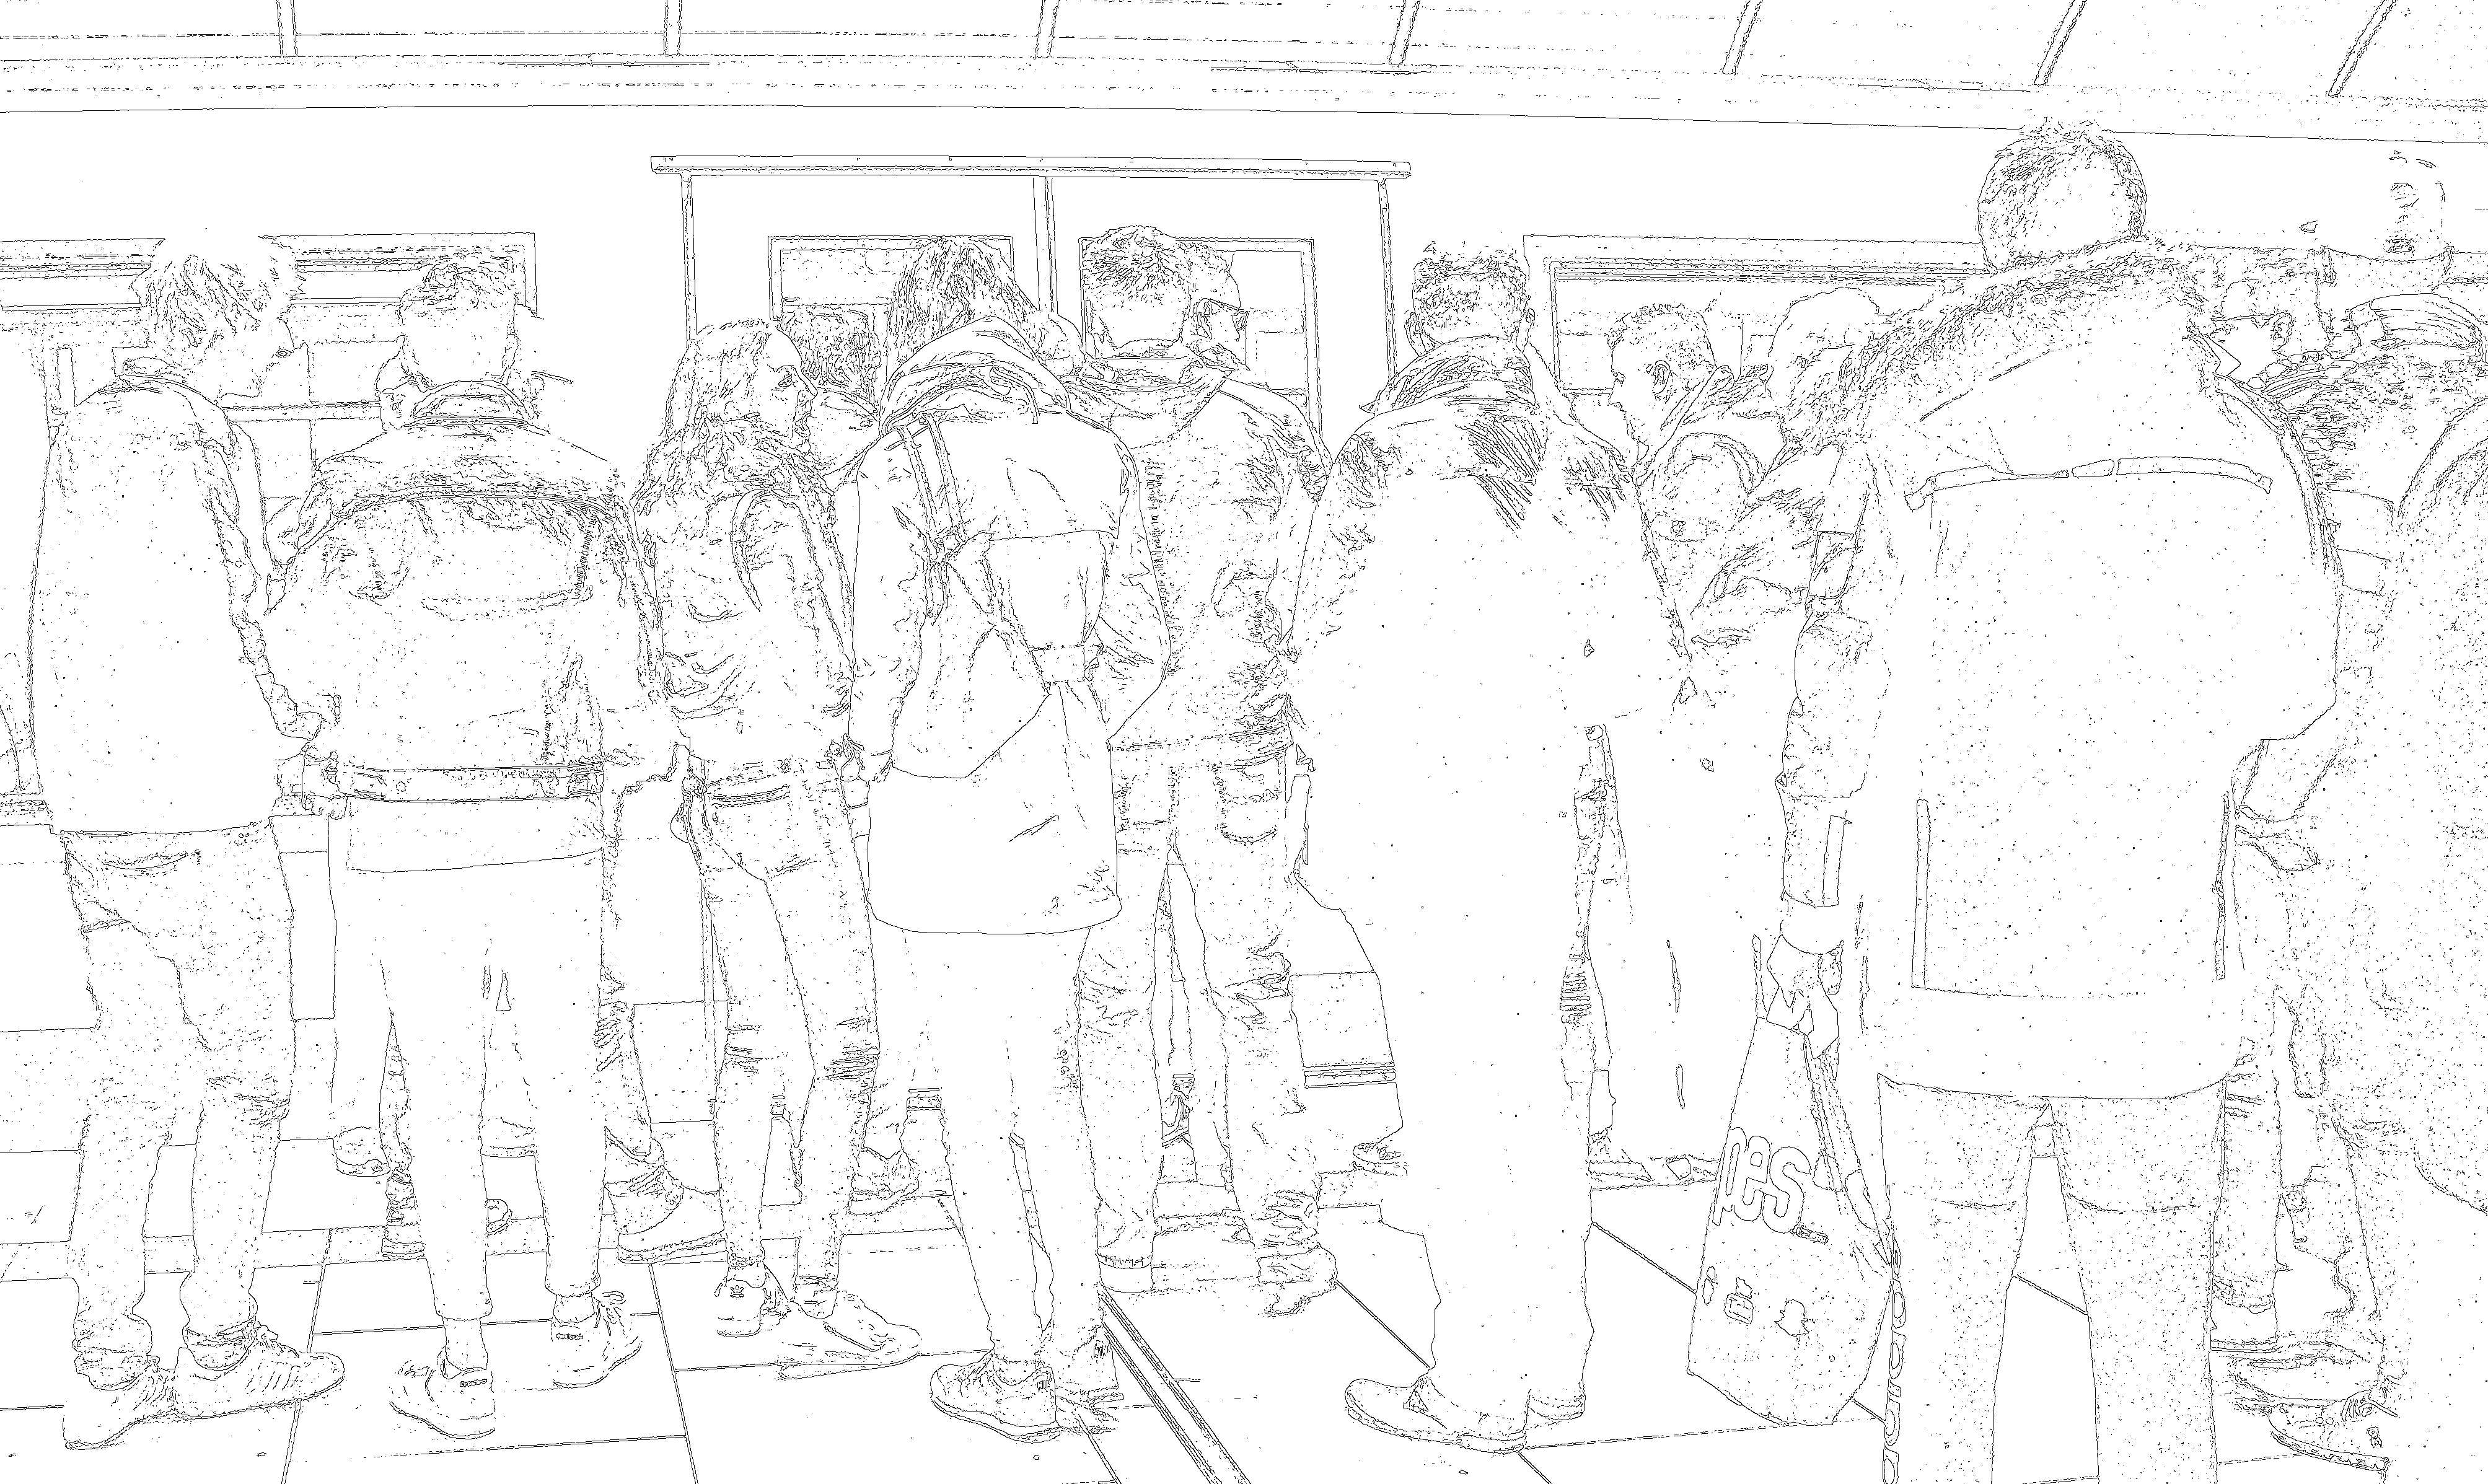
\includegraphics[width=0.8\textwidth]{pictures/observation/football/exchange_football.png}
	\caption{Fahrgastwechsel vor dem Fußballspiel, FC Bayern gegen BVB, mit wartenden Personen.}
	\label{fig:fussballFahrgastwechsel}
\end{figure}
\subsection{Einflussfaktoren}
Nachdem die Unterschiede festgestellt wurden, soll nun erklärt werden welche Einflussfaktoren diese Veränderung hervorgerufen haben könnten.
Ein Einflussfaktor für das beobachtete Verhalten könnte die andere Verteilung an Ein- und Aussteigern sein. Da nur sehr wenige Personen aus dem Zug gelangen wollen, könnte die Hemmschwelle, diesen im Weg zu stehen sinken. Dies kann jedoch nicht der einzige Grund für das andere Verhalten sein. Bei Zügen, die außerhalb des Fußballspieles beobachtet wurden und bei denen nur wenige Personen ausstiegen, wurde dieses Verhalten nicht beobachtet. Deshalb ist davon auszugehen, dass das Verhältnis nicht der einzige Grund für das im Weg stehen sein wird.\\
Um die Unterschiede erklären zu können, müssen also die beteiligten Personen genauer betrachtet werden. Einer der Unterschiede bei den Fahrgästen liegt im Alkoholkonsum. Im normalen Beobachtungszeitraum führte keiner der Fahrgäste Alkohol mit sich und keiner der Beobachteten wirkte alkoholisiert. Bei den Beobachtungen vor Beginn des Fußballspiels machten jedoch einige der Fahrgäste einen alkoholisierten Eindruck oder trugen alkoholische Getränke bei sich. Neben dem Alkoholkonsum fiel auf, dass auch die Stimmung sich bei diesen Beobachteten zu der sonstigen unterschied. Die meiste Zeit war die Stimmung aufgelöst, es wurde gesungen und U-Bahn-Wagons durch Auf- und Abspringen zum Schwanken gebracht. Diese andere Stimmung könnte ein weiterer Einflussfaktor dafür sein, dass sich das Verhalten der Passagiere verändert. \\
Die Beobachtungen zum Fußballspiel liefern interessante Ergebnisse. Da dies jedoch, in den Beobachtungen dieser Arbeit, ein absoluter Sonderfall ist, fließen sie nicht in das Modell mit ein. Eine genauere Untersuchung könnte jedoch zu einem Modell für einen solchen Spezialfall führen, welcher wiederum für eine Verbesserung der Planung der Abläufe im öffentlichen Nahverkehr führen könnte.